\chapter{Introduction} \label{chapter1}

\tab This is a very short guide to an unofficial thesis/dissertation template
for the University of Tennessee.
\mnote{Not sure when website specifications incomprehensibilities were updated.}
It is based on the 2017 thesis specifications but can be easily altered
as the guidelines are changed.
\mnote[1cm]{This is a margin note used during revisions, not the final draft.}
This template requires a basic knowledge of \LaTeX\ and should cover
the basic requirements in terms of required packages and functionality
for the University of Tennessee.
\note[green]{This is a note with custom color.}
\note{This is a note with default color.}

\begin{figure}[!htb]
    \Centering
    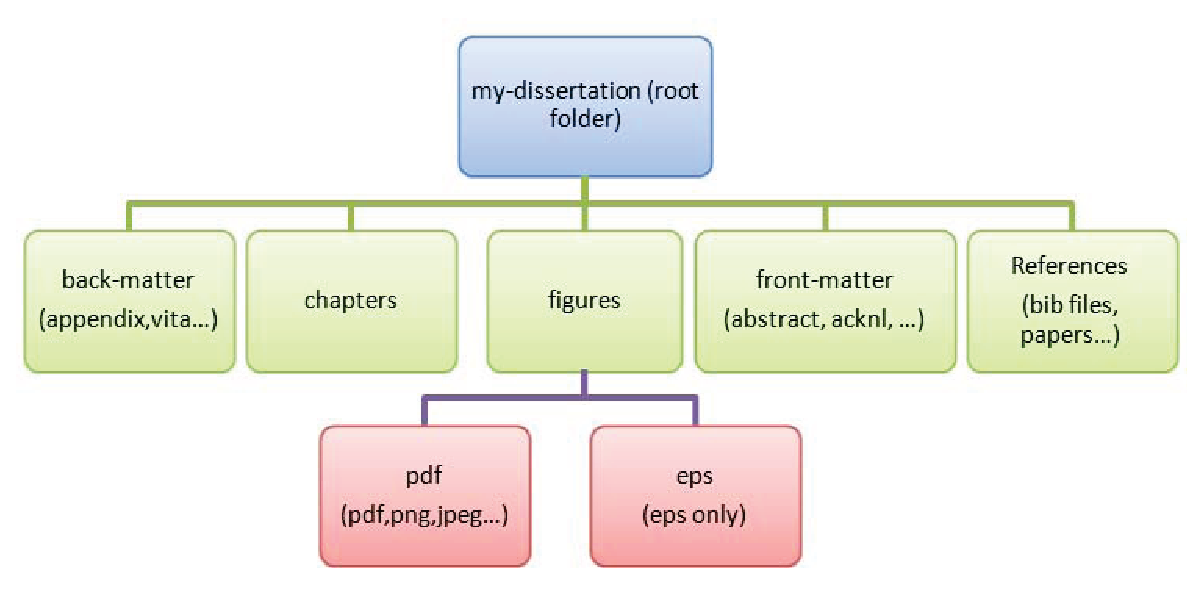
\includegraphics[width=0.9\textwidth]{fig01-folder-structure}
    \caption[UT thesis template folder structure]{UT thesis template folder structure.
        The main LaTeX file and BibTeX file are in the top directory.
        All other files are placed in any of the four folders
        (back-matter, chapters, figures, front-matter).}
    \label{fig:folderstructure}
\end{figure}

\tab The general structure of this template is based on the tree shown in
\autoref{fig:folderstructure}.
The titles of the folders are self descriptive
and should guide you to proper file placement.
Note that this is only a suggested model that could be
modified to fit your own organizational structure.

\section{A Section multiple lines} \label{asection}
This is a paragraph found in a section part.

\subsection{A subsection}
This is a paragraph found in a subsection part.
For more information, check:
\url{http://en.wikibooks.org/wiki/LaTeX/Floats,_Figures_and_Captions}

\subsection{Another subsection}
This is a paragraph found in another subsection part.

\subsubsection{A subsubsection}
This is a paragraph found in a subsubsection part.

\section{Multipart figures}
This is a paragraph found in another section part.

\begin{figure}[!htb]
    \Centering
    \begin{subfigure}[t]{0.3\textwidth}
        \Centering
        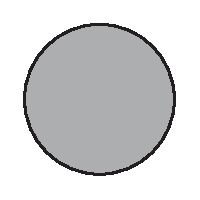
\includegraphics[width=1in]{fig02a-circle}
        \caption{\ Circle}
        \label{fig:shapes-circle}
    \end{subfigure}
    \begin{subfigure}[t]{0.3\textwidth}
        \Centering
        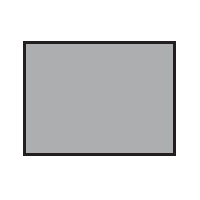
\includegraphics[width=1in]{fig02b-rectangle}
        \caption{\ Rectangle}
        \label{fig:shapes-rect}
    \end{subfigure}
    \begin{subfigure}[t]{0.3\textwidth}
        \Centering
        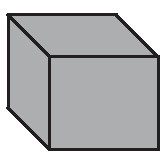
\includegraphics[width=1in]{fig02c-cube}
        \caption{\ Cube}
        \label{fig:shapes-cube}
    \end{subfigure}
    \caption[Geometric shapes]{Geometric shapes, each presented as a subfigure.
        (a) is a circle,
        (b) is a rectangle, and
        (c) is a cube.}
    \label{fig:shapes}
\end{figure}

For multipart figures (e.g., \autoref{fig:shapes-rect}),
you need to use the package ``subcaption''.

\begin{table}[!htb]
    \Centering
    \caption[Table with multiple rows]{A multirow table example.}
    \begin{tabular}{|L{3cm}|C{1cm}|C{1cm}|}
        \hline
        \textbf{col1} & \textbf{col2} & \textbf{col3} \\
        \hline
        \multirow{3}{3cm}{Multiple rows}
            & cell2 & cell3 \\
            & cell5 & cell6 \\
            & cell8 & cell9 \\
        \hline
    \end{tabular}
    \label{tab:multirow}
\end{table}

Discussing some analysis results from \autoref{tab:multirow}.
It all started at \autoref{asection} and never ended~\dots

